\documentclass[10pt,letterpaper]{article}

\usepackage{color}
\usepackage{amsmath}
\usepackage{amsfonts}
\usepackage{lmodern}
\usepackage{float}
\usepackage{placeins}
\usepackage{mathtools,xparse}
\usepackage{cite}
\usepackage{graphicx}
\usepackage[T1]{fontenc}


\DeclarePairedDelimiter{\abs}{\lvert}{\rvert}
\newcommand{\bigCI}{\mathrel{\text{\scalebox{1.07}{$\perp\mkern-10mu\perp$}}}}
\DeclareMathOperator*{\argmax}{arg\,max} 
%%%%%%%%%%%%%%%%%%%%%%% begin %%%%%%%%%%%%%%%%%%%%%%%%%%%%%%
\begin{document}
\pagenumbering{arabic}
\title{Analytic continuation of quantum Monte Carlo data via maximum entropy method}
\author{Michael Haslauer, Max Weber}

%%%%%%%%%%%%%%%%%%%%%%% References %%%%%%%%%%%%%%%%%%%%%%%%%
% \begin{thebibliography}{99}

% \end{thebibliography}
%%%%%%%%%%%%%%%%%%%%%%%%%%  body  %%%%%%%%%%%%%%%%%%%%%%%%%%

% section introduction (end)
\section{Theory} % (fold)
\label{sec:theory}
\subsection{The Maximum Entropy Method (MEM)}

Given a N dimensional noisy data set $\vec{G}$ and a model characterized by the M dimensional parameter vector $\vec{A}$. 
The model is assumed to represent a valid relation between $G_{i}$ and $\vec{A}$. This means that for an exact value $G_{i}$ 
and perhaps some other known parameters, one could in principle determine the correct vector of unknown parameters $\vec{A}$. 
However since $\vec{G}$ is noisy the uncertainty 
about the true value of $G_{i}$ induces a uncertainty on the true value of $\vec{A}$. Therefore it makes sense to determine 
a probability distribution $p(\vec{A}|\vec{G})$ instead of one single solution for $\vec{A}$. \\
Using Bayes' theorem the following relation for the wanted prob. distribution $p(\vec{A}|\vec{G})$ can be found

\begin{displaymath}
 p(\vec{A}|\vec{G}) \propto p(\vec{G}|\vec{A}) p(\vec{A})
\end{displaymath}

\noindent This is the well known $posterior \propto likelihood * prior$ relation from Bayesian statistics. Hence if it 
is possible to find the likelihood and posterior distributions one has quantitative information about the probability for 
$\vec{A}$ to be true given $\vec{G}$.\\

\subsubsection{The likelihood function}

Following Bryan [reference] for the maximum entropy method the likelihood function is restricted to the functional form 
\begin{displaymath}
 p(\vec{G}|\vec{A}) \propto exp(-L(\vec{F},\vec{G}))
\end{displaymath}
where $\vec{F}$ is leneary related to $\vec{A}$, $\vec{F} = \textbf{K} \vec{A}$ by the matrix \textbf{K} which 
represents a valid relation between $\vec{A}$ and $\vec{G}$.\\

\subsubsection{The prior distribution}

In contrast to the likelihood function which can be found by data manipulation and reasoning in most cases very exact, the 
prior is quiet hard to find in a correct way. This is the typical drawback of Bayesian inference methods.
The core of the maximum entropy method is now the used prior distribution. Following again Brayn [reference] the prior for 
an unnormalized positive additive density $\vec{A}$ is given by
\begin{displaymath}
 p(\vec{A}| \alpha, \vec{m}) \propto exp(\alpha S(\vec{m},\vec{A}))
\end{displaymath}
where $\alpha \in \mathbb{R}^+$ is a unknown parameter and S is the entropy of $\vec{A}$ relative to a default model $\vec{m}$
\begin{equation}
 S = \sum_{m=1}^{M} A_m -m_m -A_m log(A_m/m_m)
 \label{eq:S(A,m)}
\end{equation}

\noindent It is noteworthy that on the one hand this restricts the parameter vector $\vec{A}$ to be possible to be interpreted as 
\textit{positive additive density}. On the other hand the choice for $\alpha$ and $\vec{m}$ are of big influece and have to 
handled with care. This subject will be addressed in more detail in a later chapter. 

\subsubsection{The posterior distribution}

\noindent Combining now both general forms of the likelihood and prior distribution within the maximum entropy framework the posterior 
distribution for $\vec{A}$ is up to a normalization constant given by 
\begin{equation}\label{eq:posterior_general}
 p(\vec{A}|\vec{m},\alpha,\vec{G}) \propto exp(\alpha S(\vec{m},\vec{A}) - L(\vec{F},\vec{G})) = exp(Q)
\end{equation}


\noindent Hence for given $\alpha$, expression~(\ref{eq:posterior_general}) reaches its maximum probability for $\vec{\hat{A}}$
which maximizes $Q = \alpha S - L$. This means we have to find $\vec{\hat{A}}$ such that
\begin{equation}\label{eq:max_A_constraint}
 \vec{\nabla} Q(\vec{\hat{A}}) = \alpha \vec{\nabla} S(\vec{\hat{A}}) - \vec{\nabla} L(\vec{\hat{A}}) = 0
\end{equation}

\noindent The numercial solution of equation~(\ref{eq:max_A_constraint}) is the central issue of the MEM algorithm. 

\subsection{Analytic Continuation of QMC Data using MEM}

Most quantum Monte Carlo (QMC) simulations produce Green's functions $G(\tau)$ of Matsubara imaginary time $\tau = it$.
However the real time/frequency results $G(t)$/$G(\omega)$ are crucial since most experiments probe quantities related to 
the real time/frequency Green's functions. Fortunately the relation between $G(\tau)$ and the imaginary part of $G(\omega)$,
is linear and given by 
\begin{equation}\label{eq:connection_real_frequency_imag_time}
G(\tau) = \int d\omega A(\omega)K(\tau,\omega) 
\end{equation}
\noindent where the so caled Lehmann spectral function is given by $A(\omega) = -\frac{1}{\pi} \Im G(\omega)$ and $K(\tau,\omega)$ is a kernel, 
different for fermionic, bosonic or anomalous case. Therefore if it is possible to reconstruct $A(\omega)$ from given $G(\tau)$
one has the information about the real frequency Green's function $G(\omega)$. Why???? \\
In this report we will restrict our self to the fermoinic case. For fermions the Lehmann spectral function is positve 
definite, $G(\tau)$ is periodic with inverse temperatur $\beta = 1 / k_B T$ and the Kernel is given by
\begin{equation}\label{eq:ferminoc_kernel}
 K(\tau,\omega) =  \frac{exp(-\tau \omega)}{1 + exp(-\beta \omega)}
\end{equation}

\subsubsection{Discretized version of the problem}

\noindent Because of the methodically given uncertainty of Quantum Monte Carlo simulations, doing QMC for N different imaginary 
times $\tau_n$ will produce a N dimensional noisy data set $\vec{G}$ where $G_n$ is the mean of all QMC steps.\\
The idea is now to find a way to extract $A(\omega)$ form the noisy data set $\vec{G}$ using the maximum entropy method.\\
First of all we note that for the MEM formalism a valid model wich predicts $G_n$ for a given M dimensional parameter vector
$\vec{A}$ is necessary. This can be achieved if expression~(\ref{eq:connection_real_frequency_imag_time}) is approximated
as Rieman sum 
\begin{equation}
 G_n = G(\tau_n) = \int_{a}^{b} d \omega A(\omega)K(\tau_n,\omega) \approx \sum_{m=1}^M  A_m K(\tau_n,\omega_m)
\label{eq:kernel_as_reiman_sum}
\end{equation}
\noindent where $A_m = \Delta \omega A(\omega_m)$, $ \omega_m = \Delta \omega m$ and $\Delta \omega = (b-a)/M$ (a,b have to be choosen in a sensible way).
After this discretizaton we have a parameter vector $\vec{A} =(A_1,...,A_M)^T$ and a true linear model $\vec{G} = \textbf{K} 
\vec{A}$ where $\textbf{K} \in \mathbb{R}^{N\times M}$ and $K_{nm} = K(\tau_n,\omega_m)$.

\subsubsection{The likelihood function}

As already mentioned to apply the Maximum Entropy Method the likelihood function hast to have the functional form 
$ p(\vec{G}|\vec{A}) \propto exp(-L(\vec{F},\vec{G}))$ where $\vec{F}$ is leneary related to $\vec{A}$ by
$\vec{F} = \textbf{K} \vec{A}$ what is already fulfilled by~(\ref{eq:kernel_as_reiman_sum}). For QMC data it is 
possible to achieve a multivariate gaussian shape of the likelihood function, such that .
\begin{equation}
	L = 1/2 ((\vec{G} - \vec{F})^T diag\{1/ \sigma_n^2 \} (\vec{G} - \vec{F}))
	\label{eq:L(G)}
\end{equation}
Since for the purpose of this educational project work no real QMC data was available we will only give a short overview of
the main aspects how QMC data has to be manipulated in principle to reach the desired form of the likelihood function.\\
For each of the N imaginary times $\tau_n$, $G(\tau_n) = G_n$ is calculated a plenty of times in $N_{QMC}$ QMC steps, with results $G_n^i$ and each with a different error. 
Hence one can interpret the relative freqency as probability distribution \[ p_{QMC}(G_n)= n(G_n^i = G_n)/N_{QMC} \]
The resulting distribution $p_{QMC}(G_n)$ is not gaussian and also correlated between different QMC steps. To get rid
of this problem one perfoms a rebinning of the data. This means one considers the average of $n_b$ succeding measurement as new 
datapoint \[G_n^b = \sum_{(b-1) n_b + 1}^{b n_b} \frac{G_n^i}{n_b} \] 
\noindent So instead of $N_{QMC}$ datapoints for each $\tau_n$
we have now $N_b = N_{QMC}/n_b$ datapoints. This rebinning has now two desired effects wich we can understand if the
procedure is considered as logical 2 step rebinning. 
\begin{enumerate}
\item In a first rebinning we get rid of the correlations between the succeding QMC steps. (As long as the bin size $n_b$
 is choosen big enough compared to the correlation lenght.)
\item Since correlations are removed the rebinned data represents a set of independent and identical drawn random variables.
Hence for the second rebinning step we can argue using the central limit theorem that the resulting random variable should
be gaussian distributed.
\end{enumerate}

Remark: To find the optimal binsize $n_b$ the current method is to compare higher moments (skewness, kurtosis) of the rebinned 
data to a data set of equal length $N_b$, drawn by perfect gaussian. The optimal size for $n_b$ is reached if the
moments for both data samples converge.\\

\noindent This gaussian distribution can be approximated by \[ p(G_n^b) = \frac{1}{\sqrt{2 \pi} \sigma_n} exp(-\frac{(G_n^b - \overline{G}_n)^2}{2 \sigma_n^2}) \]
\noindent where $\overline{G}_n = \sum_{b} G_n^b /N_b$ and $\sigma_n^2 = \sum_b (G_n^b - \overline{G}_n)^2 / (N_b -1)$ are calculated
in the usual way from the data. It is helpfull to keep in mind, that this distributions is only an approximation and not the 
true one due to the errors in $\overline{G}_n$ and $\sigma_n$.\\
But with this information we can argue using again the CLT that the true distribution of the mean for each time step $\tau_n$ is 
again gaussian 
\[ p(\overline{G}_n) = \frac{1}{\sqrt{2 \pi} \sigma_n^{real}} exp(-\frac{(\overline{G}_n - \mu_n)^2}{2 \sigma_n^{real}}) \]

where $\mu_n$ and $\sigma_n^{real}$ represent unknown true values. We now assume that for a true $G(\tau_n)$ the observed QMC 
results are distributed in a way that $G(\tau_n)$ is given by the mean of the observed QMC results. Since the mean is conserved 
under all rebinning and averaging steps we have $G(\tau_n) = \mu_n$. Using ~(\ref{eq:kernel_as_reiman_sum}) we can argue
that for a given spectral function $A(\omega)$ the observed distribution for $\overline{G}_n$ is given by 

\[ p(\overline{G}_n | \vec{A}) = \frac{1}{\sqrt{2 \pi} \sigma_n^{real}} exp(-\frac{(\overline{G}_n - \sum_m K_{nm}A_m)^2}{2 \sigma_n^{real}}) \]

\noindent In a last step we approximate $\sigma_n^{real} \approx \sigma_n/ \sqrt N_b$ motivated by the CLT and reformulate the 
whole problem in a compact multivariate form. This gives a likelihood function 

\begin{equation}
 p(\vec{\overline{G}}|\vec{A}) \propto exp \left( -\frac{1}{2} (\vec{\overline{G}}-\textbf{K}\vec{A})^T diag\{ \frac{N_b}{\sigma_n^2} \} (\vec{\overline{G}}-\textbf{K}\vec{A})  \right)
\end{equation}

\noindent where we have assumed statistical independence between the different $\overline{G}_n$. For simplicity of notation 
we will set $\vec{\overline{G}} \rightarrow \vec{G}$ and $  \sigma_n / \sqrt N_b  \rightarrow \sigma_n$ in the upcomming parts
of this report. Such that the final form of the likelihood function given by 

\begin{align}\label{eq:likelihood function}
 \begin{split}
 p(\vec{G}|\vec{A}) & \propto  exp \left( -\frac{1}{2} (\vec{G}-\textbf{K}\vec{A})^T diag\{ \frac{1}{\sigma_n^2} \} (\vec{G}-\textbf{K}\vec{A})  \right)
 \\
 & = exp \left( -\frac{1}{2} (\vec{G}-\vec{F})^T diag\{ \frac{1}{\sigma_n^2} \} (\vec{G}-\vec{F})  \right)
 \\
 & = exp(- L(\vec{F},\vec{G}))  
 \end{split}
\end{align}

\subsubsection{The prior distribution}

Since $A(\omega)$ is positive definite $\vec{A}$ has all properties neccesary to apply the form of the MEM prior. 
\begin{equation}\label{eq:prior}
 p(\vec{A}|\alpha,\vec{m}) \propto exp(\alpha S(\vec{A},\vec{m})
\end{equation}

\subsubsection{The posterior distribution}

Putting all things together we found an expression for the probability of $\vec{A}$ to be the true spectral function in 
case observing the data $\vec{G}$ given $\alpha$ and $\vec{m}$.
\begin{equation}\label{eq:posterior}
 p(\vec{A}|\alpha,\vec{m},\vec{G}) \propto  exp(\alpha S - L(\vec{F},\vec{G})) = exp(Q(\vec{A}))
\end{equation}
Therefore for given $\alpha$ and $\vec{m}$ we can calculate the most probable $\vec{\hat{A}}$. However this tells us nothing about
the plausibility of the values for $\alpha$ and $\vec{m}$ which have significant influence of the obtained results.

\subsubsection{Approaches to treat $\alpha$}

We will present 2 common ways how to deal with the uncertainty about how to choose $\alpha$. The so called \textit{Classic} 
and \textit{Bryan's method}. 
\\
If we introduce $p(\alpha$) the prior probability distribution for $\alpha$ (which we assume to be independen on $\vec{m}$ 
we can find a posterior distribution for $\alpha$ using~(\ref{eq:posterior}) as
\begin{equation}
 p(\alpha | \vec{G},\vec{m}) = \int d\vec{A} p(\alpha,\vec{A}|\vec{G},\vec{m}) = \int d\vec{A} p(\vec{A}|\alpha,\vec{m},\vec{G})p(\alpha)
\end{equation}

\noindent Making a gaussian approximation $exp(Q(\vec{A})) \approx exp(Q(\vec{\hat{A}}) + \frac{1}{2} \delta \vec{A}^T \nabla \nabla Q(\vec{\hat{A}}) \delta \vec{A})$
of~(\ref{eq:posterior}) we can approximate the intragral by 

\begin{equation}\label{eq:prob_of_alpha}
 p(\alpha|\vec{G},\vec{m}) \propto  \prod_m  \left( \frac{\alpha}{\alpha + \lambda_m} \right)^{1/2}  exp(Q(\vec{\hat{A}}(\alpha))p(\alpha)
\end{equation}
where $\lambda_m$ are the eigenvalues of $diag\{ \vec{A}^{1/2}\} \nabla \nabla L(\vec{A}) diag\{\vec{A}^{1/2}\} $ 
evaluated at $\vec{\hat{A}}(\alpha)$.
\\
\noindent The \textit{Classic method} is now to choose $\hat{\alpha}$ which maximizes~(\ref{eq:prob_of_alpha}). Seting 
$\partial_{\alpha}p(\alpha|\vec{G},\vec{m}) = 0$ and assuming $\partial_{\alpha}\lambda_m \approx 0$ and that the prior
$p(\alpha)$ will be owerwhelmed by the data, this leads to 
\begin{equation}\label{eq:classic_method_constraint}
 -2\hat{\alpha}S \approx \sum_m \frac{\lambda_m}{\lambda_m +\hat{\alpha}} 
\end{equation}

\noindent \textit{Brayn's method} in contrast tries to use the wohle information contained in $p(\alpha|\vec{G},\vec{m})$. 
Instead of choosing one single value for $\alpha$ one takes the expection value of $\vec{\hat{A}}(\alpha)$.
\begin{equation}\label{eq:brayn_method_constraint}
 \vec{\overline{A}} = \int d\alpha \vec{\hat{A}}(\alpha) p(\alpha|\vec{G},\vec{m})
\end{equation}


% section theory (end)
\section{Numerical algorithm} % (fold)
\label{sec:numerical_algorithm}
In this section we describe the numerical algorithm to perform the analytic continuation of quantum Monte Carlo data by the maximum entropy method described by Bryan.
Also we give an overview over problems we encountered with the algorithm and modifications we propose to overcome this problems.
\subsection*{Numerical algorithm proposed by Bryan}
As described in Sec. \ref{sec:theory} the quantity $Q = \alpha S - L$ has to be maximized with respect to $\vec A$ in order to find the most probable $\vec A$ given the noisy Greens function $\vec G$.\newline
To maximize Q we calculate the gradient of Q with respect to $\vec A$ and set it to zero:
\begin{equation}
	\vec\nabla Q =  \alpha \vec\nabla S - \vec\nabla L = 0
	\label{numerical_algorithm:equ.1}
\end{equation}
Then by making use of Equ \ref{eq:S(A,m)} for $S$ and Equ. \ref{eq:L(G)} for $L$ Equ. \ref{numerical_algorithm:equ.1} leads to:
\begin{equation}
	- \alpha \log \bigg(\frac{A_i}{m_i} \bigg) = \sum K_{ji} \frac{\partial L}{\partial \vec F}
	\label{numerical_algorithm:equ.2}
\end{equation}
where:
\begin{equation}
	\vec F = \mathbf{K} \vec A \text{ and } \vec \nabla L = \frac{\partial \vec F}{\partial \vec A} \frac{\partial L}{\partial \vec F} = \mathbf{K}^T \frac{\partial L}{\partial \vec F}
	\label{numerical_algorithm:equ.3}
\end{equation}
Now, a singular value decomposition of $\mathbf{K}$ is performed with $\mathbf{K} = \mathbf{V} \mathbf{\Sigma} \mathbf{U}^T$. Please note that both $\mathbf{V}$ and $\mathbf{U}$ are orthonormal matrices and therefor $\mathbf{V}^{-1}=\mathbf{V}^T$ and $\mathbf{U}^{-1}=\mathbf{U}^T$.\newline
Then Equ. \ref{numerical_algorithm:equ.3} can be rewritten as
\begin{equation}
	-\alpha \log \bigg(\frac{\vec A}{\vec m}\bigg) = \mathbf{U} \mathbf{\Sigma} \mathbf{V}^T \frac{\partial L}{\partial \vec F} 
	\label{numerical_algorithm:equ.4}
\end{equation}
where Equ. \ref{numerical_algorithm:equ.4} has to be read component wise.
Here $\mathbf{\Sigma}$ has only components on its diagonal which are called the singular values of $\mathbf{K}$. By convention the singular values are ordered by magnitude.\newline
Defining $\vec u = \alpha^{-1} \mathbf{\Sigma} \mathbf{V}^T \frac{\partial L}{\partial \vec F}$, $\vec A$ can be represented by $\vec u$ as
\begin{equation}
	A_i = m_i \exp \Big(\sum U_{in}u_n\Big)
	\label{numerical_algorithm:equ.5}
\end{equation}
Equ. \ref{numerical_algorithm:equ.5} has the advantage that it automatically enforces positivity for $\vec A$.\newline
Now Bryan argues that unless $\mathbf{K}$ is of full rank the components of $\vec u$ will not be independent.
Because of the limited precision of the computer and the singular value decomposition some of the singular values of $\mathbf{K}$ will effectively be zero.
The search for the optimal $\vec u$ can therefor be reduced to the nonzero singular values of $\mathbf{K}$.\newline
Let $s$ be the number of nonzero singular values the search can then be limited to the $s$-dimensional space which Bryan calls the singular space. 
Bryan's method therefor first reduces all relevant matrices to the singular space.
The vector $\vec u$ is now of length $s$, the number of columns of $\mathbf{V}$ and $\mathbf{U}$ are reduced to $s$ and $\mathbf{\Sigma}$ is now a $s \times s$ square matrix.\newline
Making use of Equ. \ref{numerical_algorithm:equ.5} and $\mathbf{K} = \mathbf{V} \mathbf{\Sigma} \mathbf{U}^T$ Equ. \ref{numerical_algorithm:equ.2} can be rewritten as:
\begin{equation}
	-\alpha \mathbf{U} \vec u = \mathbf{U} \mathbf{\Sigma} \mathbf{V}^T \frac{\partial L}{\partial \vec F}
	\label{numerical_algorithm:equ.6}
\end{equation}
Multiplying Equ. \ref{numerical_algorithm:equ.6} by $\mathbf{U}^T$ on both sides it reduces to
\begin{equation}
	-\alpha \vec u = \mathbf{\Sigma} \mathbf{V}^T \frac{\partial L}{\partial \vec F} \equiv \vec g 
	\label{numerical_algorithm:equ.7}
\end{equation}
or
\begin{equation}
	-\alpha \vec u - \vec g = 0
	\label{numerical_algorithm:equ.8}
\end{equation}
Equ. \ref{numerical_algorithm:equ.8} can be solved by a multidimensional Newton search iteratively
\begin{equation}
	\mathbf{J} \vec{\delta u} = -\alpha \vec u - \vec g
	\label{numerical_algorithm:equ.9}
\end{equation}
where $\mathbf{J} = \alpha \mathbf{I} + \frac{\partial \vec g}{\partial \vec u}$ is the Jacobian and $\mathbf{I}$ the identity matrix. 
With $\mathbf{W} = \frac{\partial^2 L}{\partial^2 \vec F}$, $\mathbf{M} = \mathbf{\Sigma}\mathbf{V}^T\mathbf{W}\mathbf{V}\mathbf{\Sigma}$ and $\mathbf{T} = \mathbf{U}^T \vec A \mathbf{U}$ Equ. \ref{numerical_algorithm:equ.9} reads
\begin{equation}
	((\alpha + \mu) \mathbf{I} + \mathbf{M}\mathbf{T}) \vec{\delta u} = -\alpha \vec u - \vec g
	\label{numerical_algorithm:equ.10}
\end{equation}
At each iteration step of the Newton search the step length $\vec{\delta u}$ muss be restricted for the stability of the algorithm.
Therefor, a Levenberg-Marquardt parameter $\mu$ is added in Equ. \ref{numerical_algorithm:equ.10} to ensure stability.\newline
Bryan proposes 
\begin{equation}
	\vec{\delta u}^T \frac{\partial \vec A}{\partial \vec u}\mathbf{diag}\{\frac{1}{A_i}\}\frac{\partial \vec A}{\partial \vec u}
	\vec{\delta u}^T = \vec{\delta u}^T \mathbf{T} \vec{\delta u} \leq \sum m_i
	\label{numerical_algorithm:Bryans_norm}
\end{equation}
as a maximum step length for the algorithm.\newline
Now the Newton search can be made more efficient by diagonalizing Equ. \ref{numerical_algorithm:equ.10}. First we diagonalize $\mathbf{T}$:
\begin{equation}
	\begin{gathered}
		\mathbf{T} \mathbf{P} = \mathbf{P} \mathbf{\Gamma},\\
		\mathbf{\Gamma} = \mathbf{diag} \{\gamma_i\}
	\end{gathered}
	\label{numerical_algorithm:equ.11}
\end{equation}
Then we define
\begin{equation}
	\mathbf{B} = \mathbf{diag} \{ \gamma_i^{\frac{1}{2}}\}\mathbf{P}^T \mathbf{M}\mathbf{P}\mathbf{diag}\{ \gamma_i^{\frac{1}{2}}\}
	\label{numerical_algorithm:equ.12}
\end{equation}
and again solve the eigenvalue equation
\begin{equation}
	\begin{gathered}
		\mathbf{B} \mathbf{R} = \mathbf{R} \mathbf{\Lambda},\\
		\mathbf{\Lambda} = \mathbf{diag} \{\lambda_i\}
	\end{gathered}
	\label{numerical_algorithm:equ.13}
\end{equation}
Please note that $\mathbf{P}$ and $\mathbf{R}$ are orthogonal matrices and $\gamma_i$ and $\lambda_i$ the eigenvalues of $\mathbf{T}$ and $\mathbf{B}$. Then to diagonalize Equ. \ref{numerical_algorithm:equ.10} we define 
\begin{equation}
	\mathbf{Y} = \mathbf{P} \mathbf{diag}\{ \gamma_i^{-\frac{1}{2}}\} \mathbf{R}
	\label{numerical_algorithm:equ.14}
\end{equation}
With $\mathbf{Y}^{-T}\mathbf{Y}^{-1} = \mathbf{T}$ and $\mathbf{Y}^{-1}\mathbf{M}\mathbf{Y}^{-T} = \mathbf{\Lambda}$ Equ. 
\ref{numerical_algorithm:equ.10}
can be rewritten as
\begin{equation}
	[( \alpha + \mu) \mathbf{I} +\mathbf{\Lambda}]\mathbf{Y}^{-1} \vec{\delta u} = \mathbf{Y}^{-1}[ -\alpha \vec u - \vec g]
	\label{numerical_algorithm:equ.15}
\end{equation}
which leads to s independent equations for $\mathbf{Y}^{-1} \vec{\delta u}$.
Now Equ. \ref{numerical_algorithm:equ.10} can be rewritten to
\begin{equation}
	(\alpha + \mu)\vec{\delta u} = -\alpha \vec u - g - \mathbf{M}\mathbf{Y}^{-T}\mathbf{Y}^{-1} \vec{\delta u}
	\label{numerical_algorithm:equ.16}
\end{equation}
So to finally we first solve Equ. \ref{numerical_algorithm:equ.15} for $\mathbf{Y}^{-1} \vec{\delta u}$, use it in Equ. \ref{numerical_algorithm:equ.16} to solve for $\vec{\delta u}$ and calculate the new value for $\vec u_{n+1} = \vec u_{n} + \vec{\delta u}$. The iteration is terminated if $\sum_i |\vec u_{n+1} - \vec u_{n}| \leq 10^{-8}$. There exists however no deeper motivation for this criterion. 
We choose this value both for the sake of fast convergence and because we have seen no situations where the results of the algorithm improve further for lower values.\newline
We should notice that in practice Equ. \ref{numerical_algorithm:equ.14} can be ill defined due to very small $\gamma_i$ values. But only $\mathbf{Y}^{-1}$ is needed in all the calculations and it is straight forward to find the expression $\mathbf{Y}^{-1} = \mathbf{R}^T \mathbf{diag} \{ \gamma_i^{\frac{1}{2}}\}\mathbf{P}^T$ because of the orthogonality of $\mathbf{P}$ and $\mathbf{R}$.
\subsection*{Difficulties with the algorithm and proposed solutions}
Now we describe the difficulties due to numerical instabilities we had with the algorithm and propose solutions to overcome these.
\subsubsection*{Numerical overflow in $\vec A$}
In every iteration step of the newton search we calculate $\vec A$ according to Equ. \ref{numerical_algorithm:equ.5}.
Due to the exponential there is a risk of numerical overflow due to large step sizes $\vec{\delta u}$. 
We found that often even if Equ. \ref{numerical_algorithm:Bryans_norm} is fulfilled the algorithm can be instable due to numerical overflow in $\vec A$.
The reason for this we assume to be the invalid linear approximation of $\vec {\delta A} = \mathbf{U}^T \vec A\vec{\delta u}$, i.e. $\vec{\delta A} << \vec A(\vec u + \vec{\delta u}) - \vec A(\vec u)$. 
Therefor, we use the criterion $\parallel \vec{\delta A} \parallel^2 \leq \sum_i m_i$.
\subsubsection*{Eigenvalue computation}
Often we encountered complex eigenvalues returned by the numpy.linalg.eig routine for symmetric matrices.
As the eigenvalues of a symmetric real matrix have to be real we suspect this to be a issue with the standard eigenvalue computation routine of numpy.
After using the numpy.linalg.eigh routine which enforces real eigenvalues for symmetric matrices we managed to get rid of this problem.
Furthermore in some cases one of the eigenvalues of $\mathbf{T}$ was negative. This causes a problem in the square root in Eq. \ref{numerical_algorithm:equ.12}. Because this negative eigenvalue was very small (of the order of $10^{-14}$) we set it to zero if it occurred. We suspect the reason for this value to be due to numerical errors in the eigenvalue calculation routine especially because of its low magnitude.
\subsubsection*{Lewenberg-Marquardt parameter}
Unfortunately, both Bryan and Jarrell give no indication on how to choose the Lewenberg-Marquardt parameter for the newton search $\mu$.
Clearly it is reasonable to choose a value of $\mu$ driven by data.
Therefor, we motivate our choice of $\mu$ by the following idea:\newline
For large values of $\mu$ the Newton search becomes the method of steepest descent ($\mu >> \alpha: (\mu \mathbf{I} + \mathbf{J})\vec{\delta u} = \nabla Q \rightarrow \mu \mathbf{I} \vec{\delta u} = \nabla Q$). Independent of this limit the method for steepest descent reads as $\vec{\delta u} = h \nabla Q$. Therefor, we can identify $\mu$ as $h^{-1}$.\newline
As the method of steepest descent is a first order approximation algorithm we need to choose $h$ in a way that this approximation stays valid. We therefor demand that the relative error $r$ caused by neglecting the second order terms should be equal to 0.1. We calculate r by $r = (h\nabla Q^T \mathbf{J}\nabla Q)^{-1}\nabla Q^T\nabla Q$. This equation gives us the needed relation between $r$ and $h$ and therefor also $\mu$.
\subsubsection*{MEM for weak noise}
During our investigation of MEM we encountered a high numerical instability of the method especially for low values of the relative standard deviation of the Gaussian noise distribution $\sigma$.
The algorithm  ``crashed'' due to numerical overflow in $\vec A$ although we applied our improved criterion for the maximum step length $\parallel \vec{\delta A} \parallel^2 \leq \sum_i m_i$.
We at least partly suspect the reason for that to be the matrix $\mathbf{W} = \mathbf{diag}((\sigma G(\tau))^{-2})$ which has already elements of the order of $10^{14}$ for $\sigma = 10^{-4}$.
This behavior is highly counter intuitive at first because for ``improving'' data numerical instabilities arise.
At the times when Bryan proposed this algorithm and Jarrell adapted it for analytic continuation of Quantum Monte Carlo data, the accessible accuracies for the data were supposedly much lower than they are nowadays. We simply expect this to be the reason that neither Bryan of Jarell address this issue and restrict ourselves to a maximum accuracy of $\sigma = 10^{-4}$.
\subsubsection*{Impact of $\alpha$}
Ab interesting property rather than a problem worth mentioning is that the stability of the algorithm is dependent on $\alpha$.
In some cases it is possible even for relatively small error bars to stabilize the algorithm by choosing a large alpha.
But this gives rise to the problem that we cannot estimate the spectrum $A(\omega$ over a large range of $\alpha$ independent of the noise present in the data.
In this case we can only propose solutions for single values or over small ranges of $\alpha$.
However, we find this fact worth mentioning because we found empirically that the resulting spectra tend to not change much for increasing $\alpha$ after a certain value. Therefor, if one needs to get a result for data which causes instabilities in the algorithm it could be worth trying to increase $\alpha$ to stabilize it.

% section numerical_algorithm (end)
\section{Results} % (fold)
\label{sec:results}
In this section we investigate the performance of the MEM by applying it to synthetic Greens function in order to recover the spectrum $A(\omega)$. We generate the Greens function data by first calculating the spectrum $A(\omega)$ and then using Equ. \ref{eq:kernel_as_reiman_sum} to calculate the Greens function given our spectrum and the kernel $K(\tau,\omega)$. After that we corrupt the Greens function by relative Gaussian noise as the ``real'' Greens function obtained by Quantum Monte Carlo methods always suffers from noise. This distribution of noise ensures the properties get the assumed shape of L. In this evaluation we solely use the spectrum of the BCS superconductor for our investigation which can be calculated as
\begin{equation}
	A(\omega) = 
		\begin{cases}
			\frac{1}{W} \frac{|\omega|}{\sqrt{\omega^2 - \Delta^2}}&, \text{ if } \Delta < |\omega| < \frac{W}{2} \\
			0 &, \text{else}
		\end{cases}
	\label{results:equ.1}
\end{equation}
where $W$ denotes the bandwidth and $2\Delta$ the gap magnitude. We vary $\omega$ from 0 to 10 in 800 steps and $\tau$ from 0 to $\frac{\beta}{2}$ in 1000 steps for $\beta = 10$. The spectrum of the BCS superconductor is chosen because it contains a flat region, one steep peak and a sharp gap edge. This variety of features makes the spectrum an ideal test case.
In Fig. we show an example of the spectrum and the resulting Greens function for $W = 0.9$ and $\Delta = 10$.
\begin{figure}[htbp]
	\centering
	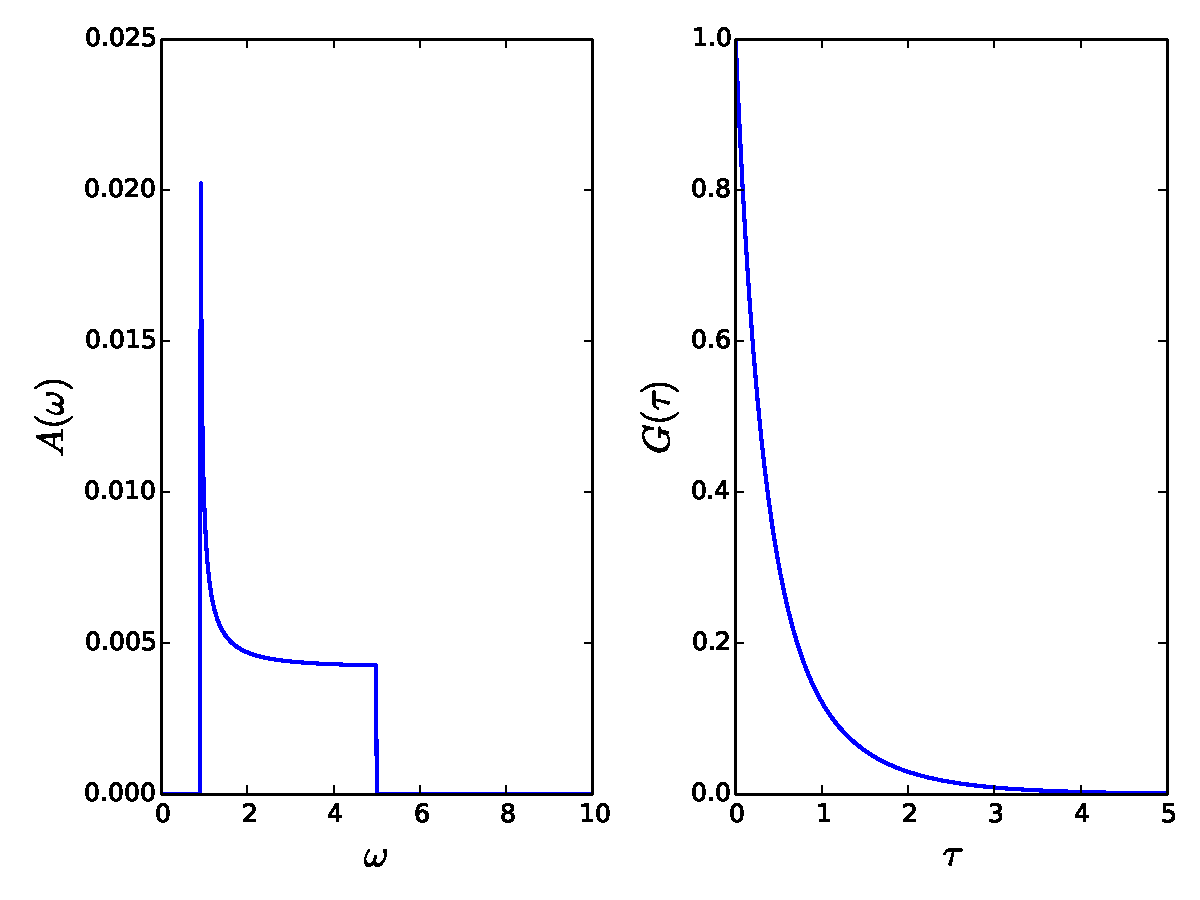
\includegraphics[width=0.95\textwidth]{./images/BCS_A_G_example.pdf}
	\caption{Example BCS spectrum $A(\omega)$ (left) and resulting Greens function $G(\tau)$ (right). The spectrum is calculated according to Equ. \ref{results:equ.1} with $\Delta = 0.9$ and $W = 10$.}
	\label{results:fig.1}
\end{figure}
\FloatBarrier
\subsection*{Influence of $\alpha$}
In the following we investigate the influence of $\alpha$.
We found that the results obtained by MEM highly depend on the regularization parameter $\alpha$. We demonstrate the influence of $\alpha$ by estimating the spectrum shown in Fig. \ref{results:fig.1} for three different values for $\alpha = 0.5,5,50$. The results are shown in Fig. \ref{results:fig.2}
\begin{figure}[htbp]
	\centering
	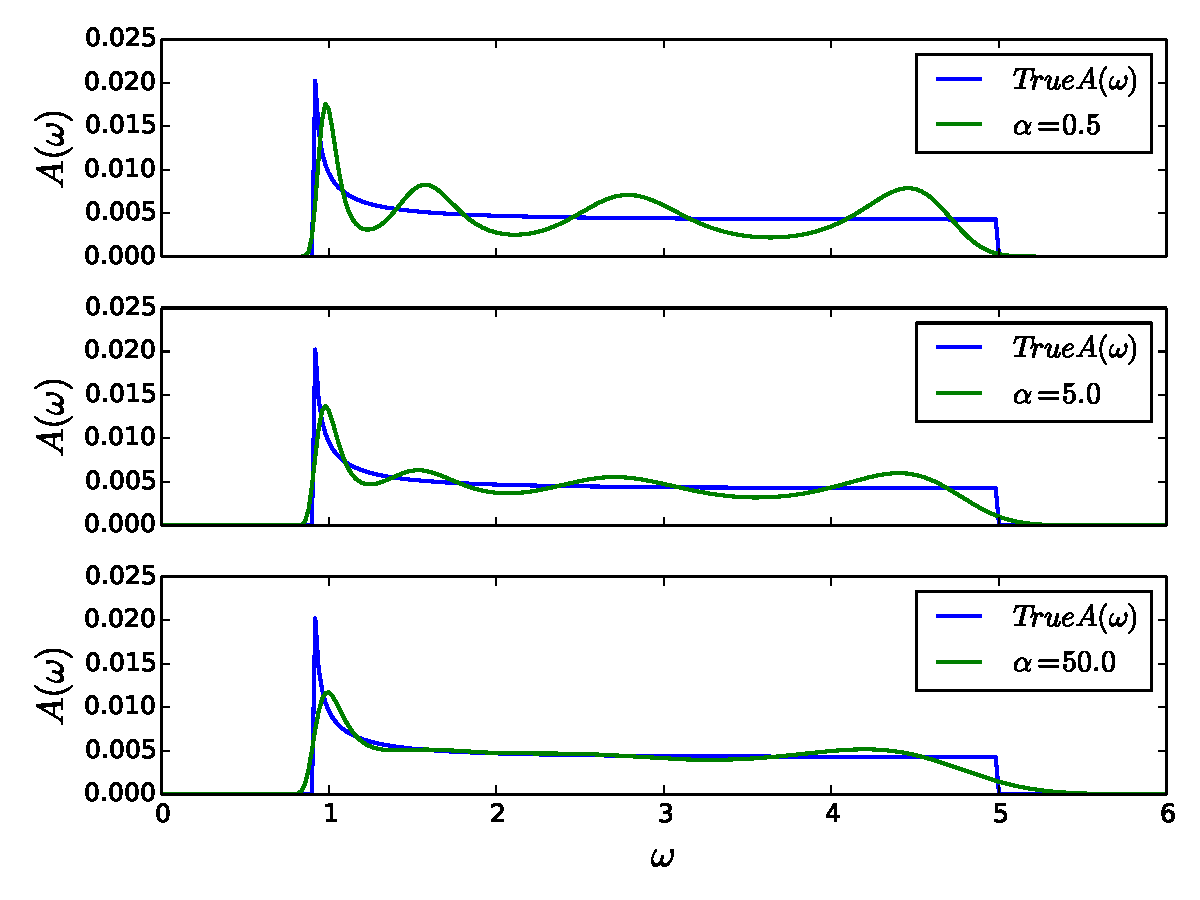
\includegraphics[width=0.95\textwidth]{./images/BCS_varying_alpha.pdf}
	\caption{Influence of the regularization parameter $\alpha$ on the performance of the Maximum Entropy method. The spectrum is calculated according to Equ. \ref{results:equ.1} with $\Delta = 0.9$ and $W = 10$.}
	\label{results:fig.2}
\end{figure}
\FloatBarrier
We observe that for increasing values of $\alpha$ the oscillation like features in the flat region of the spectrum start to vanish and therefor result in a better approximation of the real spectrum in this region. In contrast, the sharp peak at the beginning of the spectrum gets resolved worse for larger values of $\alpha$. This result resembles very nicely the impact of the regularization parameter $\alpha$ on the resulting estimated spectrum. The oscillations due to noise get suppressed at the cost of loosing features like the sharp peak at the beginning of the real spectrum. We further notice that for all three $\alpha$-values the sharp edge at the right end of the spectrum is not resolved very well.
\subsection*{Influence of the singular value threshold $\theta$}
Another important parameter is the choice of the minimum singular value $\theta$ which determines the dimension of the singular space.
Next we investigate the impact of $\theta$ on the performance of the Maximum Entropy method in Fig. \ref{results:fig.3}
\begin{figure}[htbp]
	\centering
	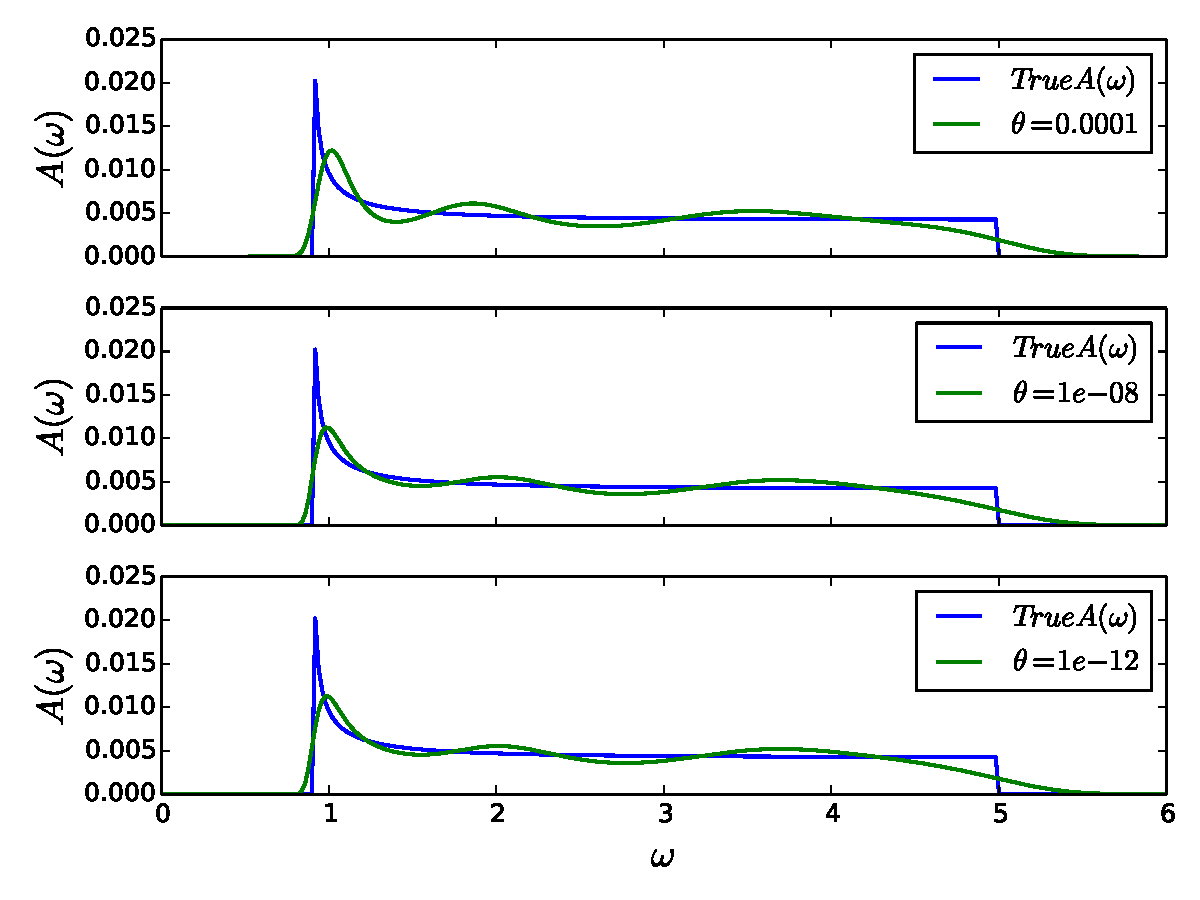
\includegraphics[width=0.95\textwidth]{./images/BCS_varying_cutoffs.pdf}
	\caption{Influence of the minimum singular value $\theta$ on the performance of the Maximum Entropy method. The spectrum is calculated according to Equ. \ref{results:equ.1} with $\Delta = 0.9$ and $W = 10$ and shown in blue in every subplot.}
	\label{results:fig.3}
\end{figure}
\FloatBarrier
Here we see that choosing a very high value for $\theta = 10^{-2}$ results in a wrong approximation of the true spectrum. Whereas reducing $\theta$ to $10^{-3}$ already results in a great improvement on the estimated spectrum. For smaller values of $\theta = 10^{-5},10^{-10},10^{-15}$ there are practically no differences while we can observe that for all of this values the first peak of the BCS spectrum gets resolved better than for $\theta = 10^{-3}$.\

\subsection*{Approaches for $\alpha$}

Now we show the difference between classic MEM and the Bryan method in choosing $\alpha$. As discussed in the theory part the classic MEM uses the maximum value of the probability of $\alpha$ given $A$ and $G$ while Bryan calculates the final $\hat{A}$ by  $\hat{A} = \int A(\alpha) P_{\alpha} d\alpha$. In Fig.~\ref{results:fig.4} we show the probability $p_{\alpha}$ and the resulting spectra calculated by classic and Bryan's method
\begin{figure}[htbp]
	\centering
	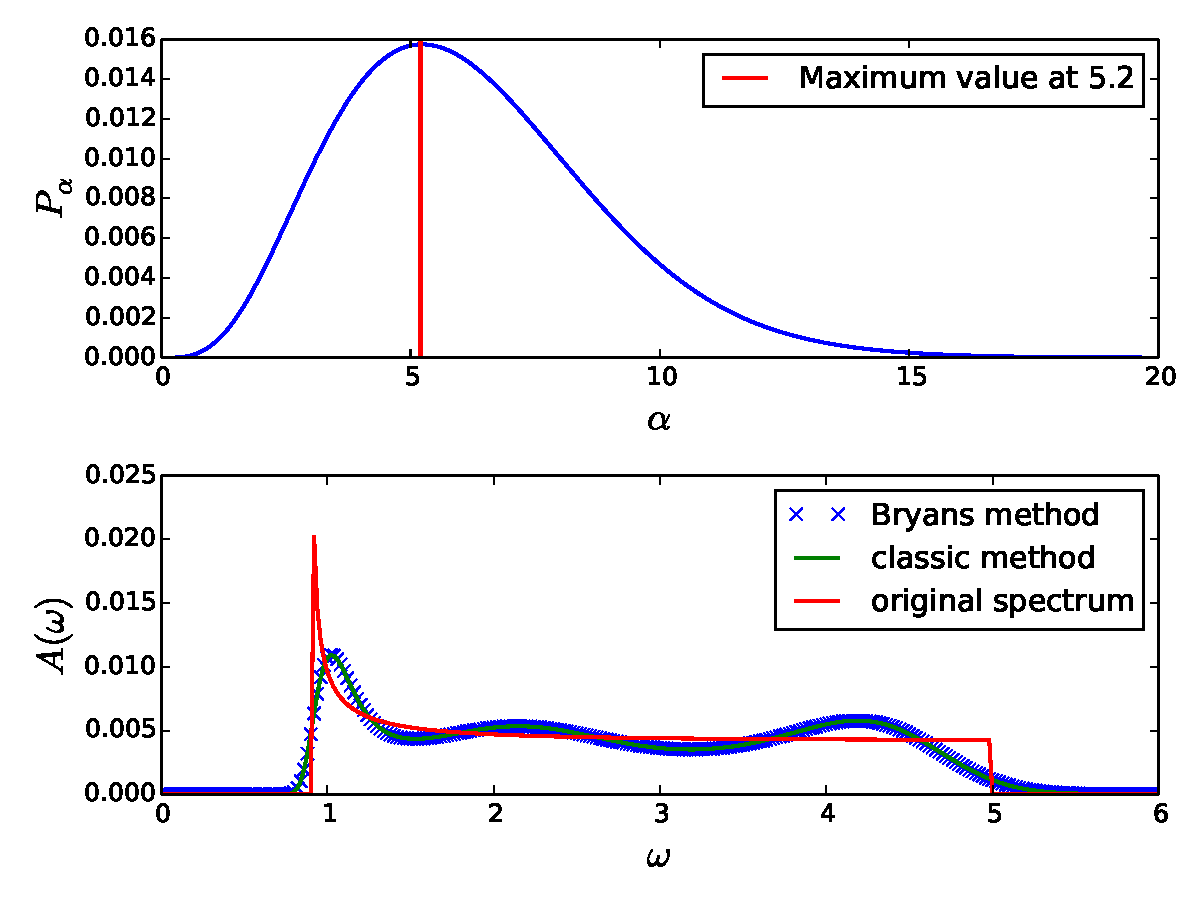
\includegraphics[width=0.95\textwidth]{./images/BCS_Bryan_classic_p_alpha.pdf}
	\caption{Upper row: probability distribution of $\alpha$ for steps of 0.1 in $\alpha$ from 0.5 to 20. lower row: resulting spectra using the classic method and Bryan's method}
	\label{results:fig.4}
\end{figure}
\FloatBarrier
There is practically no visible difference between the classic method and Bryan's method for this data. We suspect this to be at least partly due to the fact, that for $\alpha$ values larger and equal the maximum value of $P_{\alpha}$ the resulting spectra do not change much and only for small values of $\alpha$ we see significant differences in the resulting spectrum. We therefor will perform all following calculations at a constant value of $\alpha = 5$.
We have found empiricaly that this value lies always in the region where a change in $\alpha$ has nearly no influence on the resulting spectrum.
\subsection*{Influence of the noise}
Next we demonstrate the influence of the relative noise in the green's function $G(\tau)$. We estimate the spectra for four different standard deviations of the noise from $10^{-1}$ to $10^{-4}$. To get comparable results we use always the same noise sample  multiplied by the respective relative noise strengths.The results are shown in Fig. \ref{results:fig_5}
\begin{figure}[htbp]
	\centering
	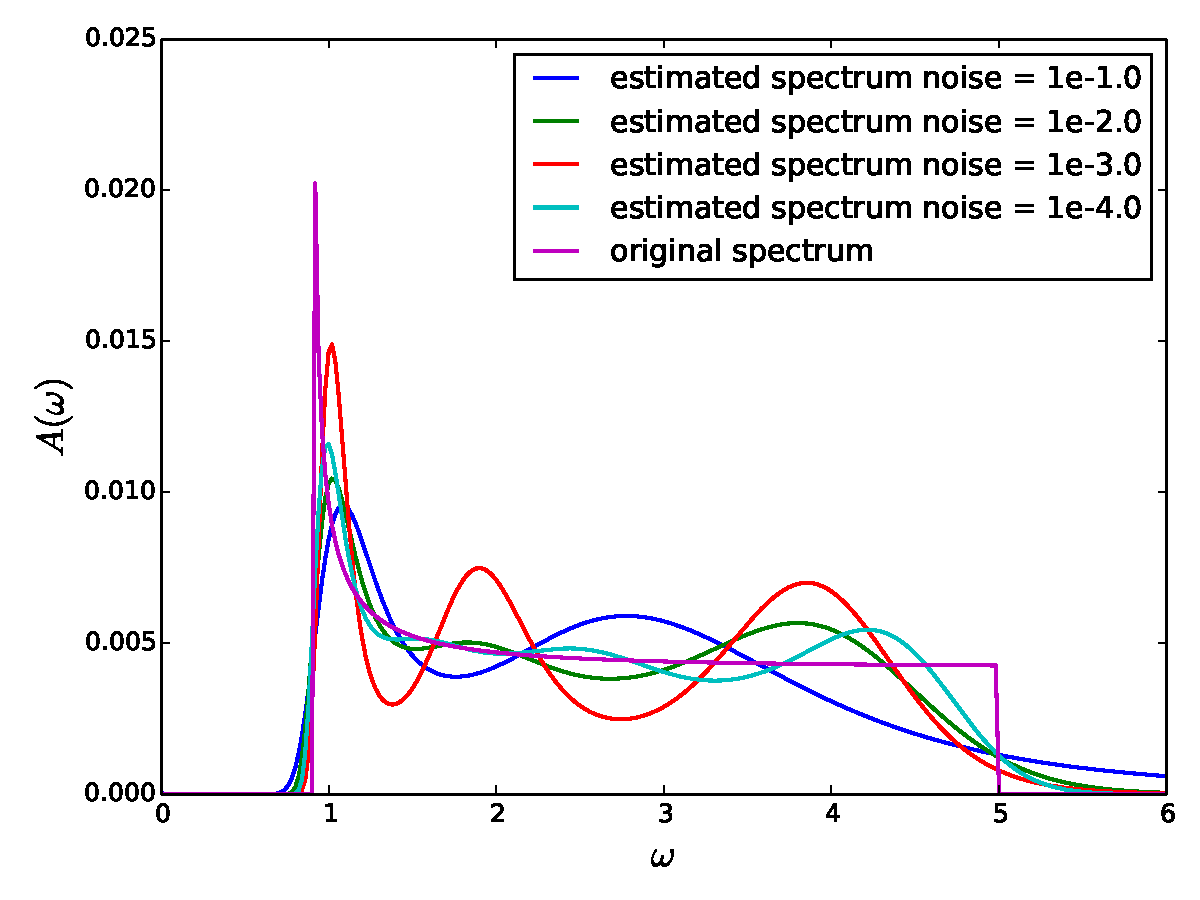
\includegraphics[width=0.95\textwidth]{./images/BCS_varying_noise.pdf}
	\caption{Resulting spectra $A(\omega)$ for four different noise standard deviations.}
	\label{results:fig_5}
\end{figure}
\FloatBarrier
As one would expect in general the estimation of the spectrum becomes better for decreasing noise. For a standard deviation of 10\% of the true greens function data we hardly recover the main features of the true spectrum. For values of 1\%, 0.1\%  and 0.01\% the sharp peak at the beginning and the edge at the right end of the true spectrum becomes more and more captured by the estimated spectrum.

\subsection*{Influence of the default model}
Finally we investigate the impact of the default model $\vec m$ on the performance of the MEM. On the one hand we show the difference for two noninformative, i.e. constant, models which differ only by a constant factor of 10. On the other hand we introduce information about the true spectrum in $\vec m$ to see if we can achieve more accurate results by this. For example if the gap width $\Delta$ of the BCS spectrum is known one could include this information into the default model $\vec m$. We implement this case by adding a delta peak at the frequency value which maximizes true spectrum on top of the noninformative constant $\vec m$. We show the used default models $\vec m$ in Fig. 6 and the results obtained by using them in Fig. \ref{results:fig_7}
\begin{figure}[htbp]
	\centering
	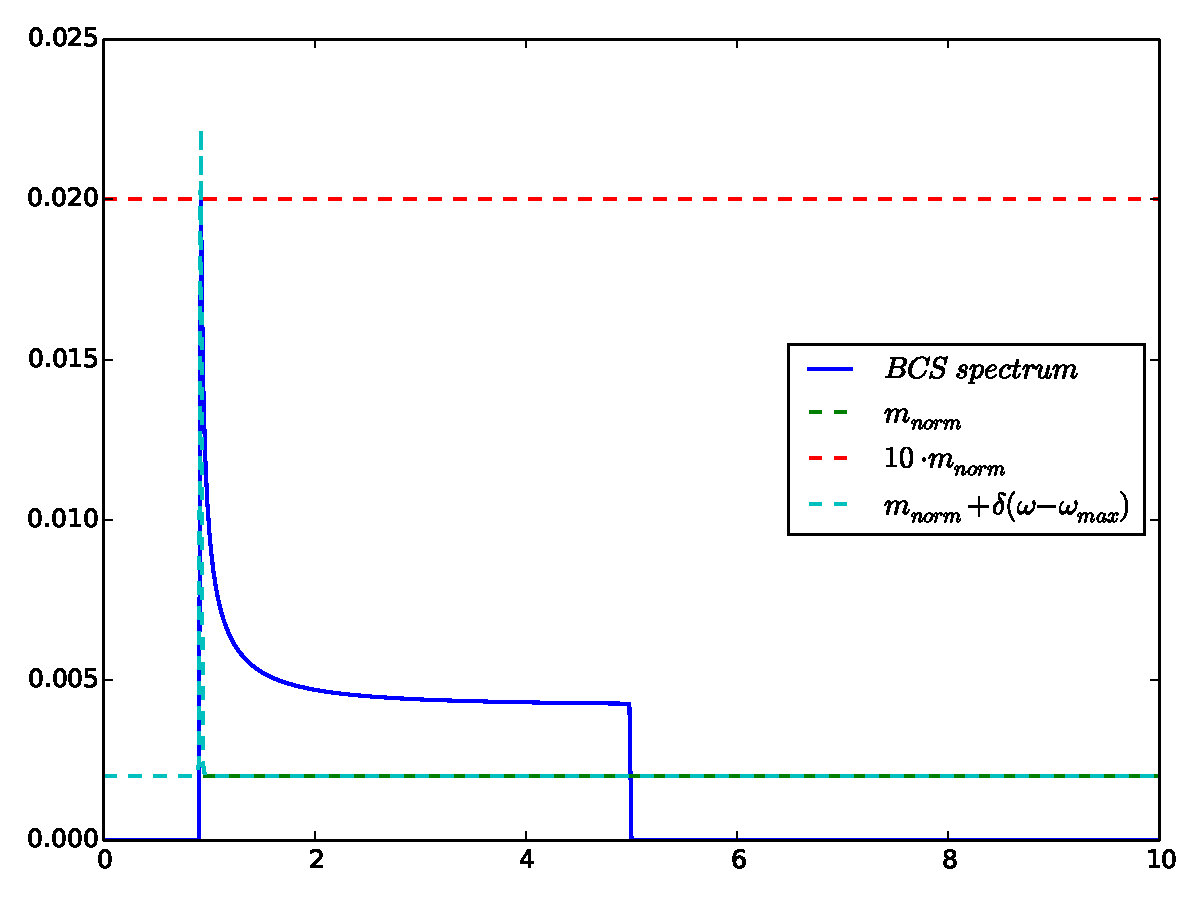
\includegraphics[width=0.95\textwidth]{./images/BCS_different_default_models.pdf}
	\caption{Illustration of the different default models $\vec m$ used.}
	\label{results:fig_6}
\end{figure}
\FloatBarrier
\begin{figure}[htbp]
	\centering
	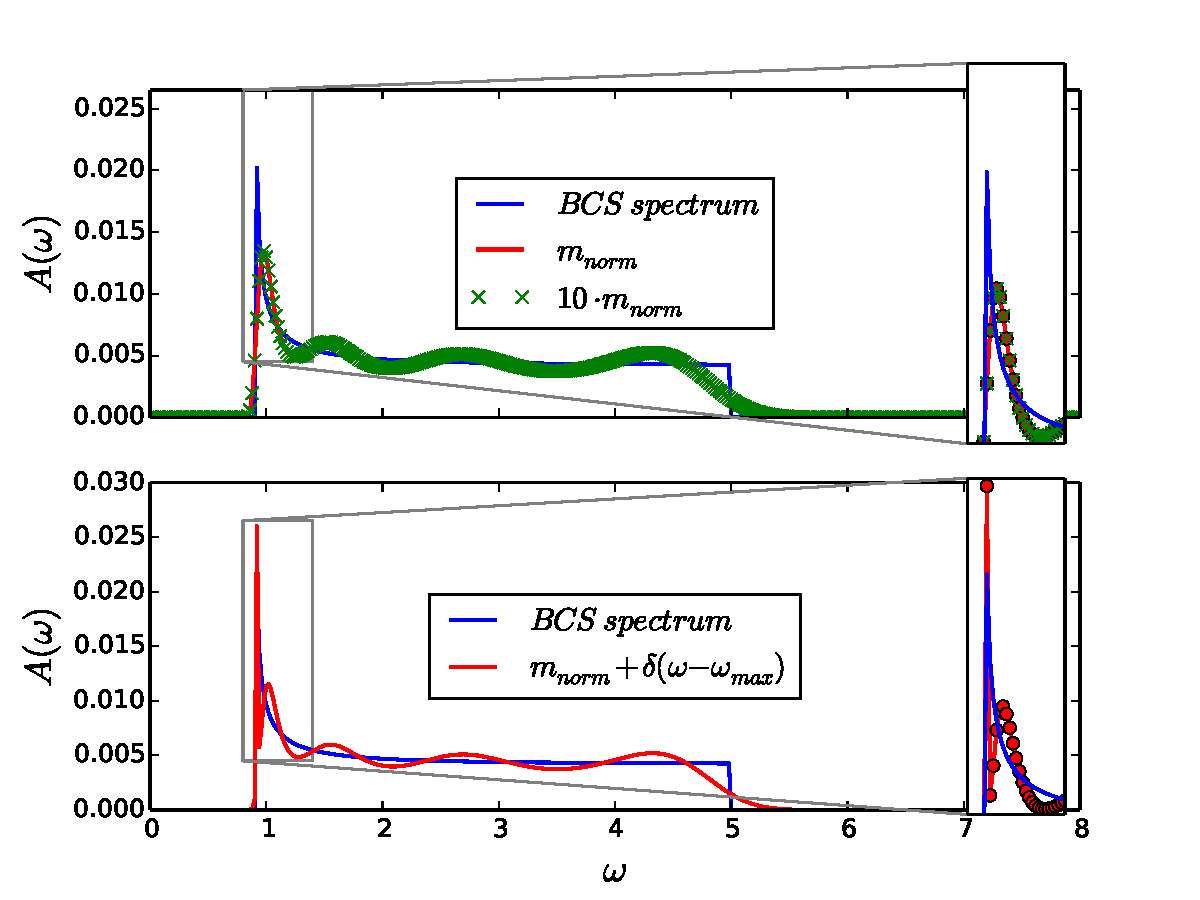
\includegraphics[width=0.95\textwidth]{./images/BCS_delta_peak_example.pdf}
	\caption{Illustration of the effect of $\vec m$ on the performance of the MEM.}
	\label{results:fig_7}
\end{figure}
\FloatBarrier
Surprisingly multiplying $\vec m$ by 10 has no impact on the resulting spectrum (upper plot). This allows us to argue that as long as no information about the true spectrum is known choosing a normalized constant default model is sufficient.
Introducing information in form of a delta peak at the gap width results in a sharp peak at the correct position of the original spectrum. However, one hast to be careful since such strong information as a delta peak will always appear in the estimated spectrum.

% section results (end)
\section{Conclusions} % (fold)
\label{sec:conclusions}
% section conclusions (end)
\end{document}
